\documentclass[10pt,a4paper,twocolumn]{article}
\usepackage[margin=19mm,columnsep=7mm,headheight=12pt,headsep=6mm,footskip=9mm]{geometry}
\usepackage{lmodern,amsmath,amssymb,graphicx,booktabs,array}
\usepackage{xcolor,caption,titlesec,fancyhdr,xurl,balance}
\usepackage[colorlinks=true,linkcolor=teal,citecolor=teal,urlcolor=teal]{hyperref}
\definecolor{navy}{HTML}{182D45}
\definecolor{teal}{HTML}{147D83}
\hypersetup{pdftitle={Probing Computation with Representation Geometry: Evidence and Limits from RaspFormer},pdfauthor={RaspFormer project},pdfsubject={Concise research paper on PR, CKA, and controlled computation-recovery experiments}}
\setlength{\parindent}{1em}
\setlength{\parskip}{2pt}
\setlength{\tabcolsep}{5pt}
\renewcommand{\arraystretch}{1.13}
\setlength{\emergencystretch}{1.5em}
\captionsetup{font=small,labelfont=bf,labelsep=period,skip=5pt}
\titleformat{\section}{\sffamily\normalsize\bfseries\color{navy}}{\thesection}{.5em}{}
\titleformat{\subsection}{\normalsize\bfseries}{\thesubsection}{.5em}{}
\titlespacing*{\section}{0pt}{8pt}{4pt}
\titlespacing*{\subsection}{0pt}{6pt}{2pt}
\raggedbottom
\pagestyle{fancy}
\fancyhf{}
\fancyhead[L]{\sffamily\footnotesize RaspFormer: representation geometry and computation}
\fancyhead[R]{\sffamily\footnotesize Research note}
\fancyfoot[C]{\footnotesize\thepage}
\renewcommand{\headrulewidth}{.3pt}
\newcommand{\PR}{\operatorname{PR}}
\newcommand{\CKA}{\operatorname{CKA}}
\newcommand{\lead}[1]{\noindent\textbf{#1}}
\title{\vspace{-10mm}\sffamily\bfseries\Large Probing Computation with Representation Geometry:\\Evidence and Limits from RaspFormer}
\author{\normalsize RaspFormer project}
\date{\small 17 October 2026}

\begin{document}
\twocolumn[\maketitle\vspace{-7mm}
\begin{center}\begin{minipage}{.94\textwidth}
\small\textbf{Abstract.}
Can representation geometry reveal computation beyond confirming a compiler's known encoding? We evaluate participation ratio (PR) and linear centered kernel alignment (CKA) on twelve RASP programs, nine structural variants, and 36 trained transformers. Controls include numerical variance filtering, orthogonal rotation, executing residual compression, geometry-directed interventions, and blind first-write detection. On six held-out programs, PR and CKA detectors achieve macro F1 of 0.853 and 0.850, versus 0.745 for always predicting a write. However, random half-width compression attains CKA schedule F1 of 0.879 while task accuracy falls to 37.6\%. PCA patches outperform random directions descriptively, but named-variable mapping requires supervision. Geometry therefore provides partial execution-timing evidence; it does not identify complete algorithms or guarantee preserved computation.
\par\vspace{2mm}\textbf{Keywords:} mechanistic interpretability; compiled transformers; participation ratio; CKA; causal interventions.
\end{minipage}\end{center}\vspace{3mm}]
\thispagestyle{plain}

\section{Introduction}
Tracr compiles RASP programs into transformers with known structure for controlled interpretability experiments~\cite{tracr}. Agreement with a known representation does not establish independent computation discovery.

Original RaspFormer independently evaluates intermediate RASP values but encodes them with compiler-known lanes and write times. Agreement measures compiler fidelity. PR also depends on encoding: a centered, balanced, equally scaled one-hot variable with $k>1$ categories has PR $k-1$. One-variable programs P01, P02, and P03 therefore give 5, 1, and 12; dimensionality alone is not algorithmic complexity.

We test numerical artifacts, program structure, coordinate changes, causal patches, and trained models. Blind prediction withholds compiler coordinates and write schedules. Negative results are retained.

\begin{figure*}[t]
\centering
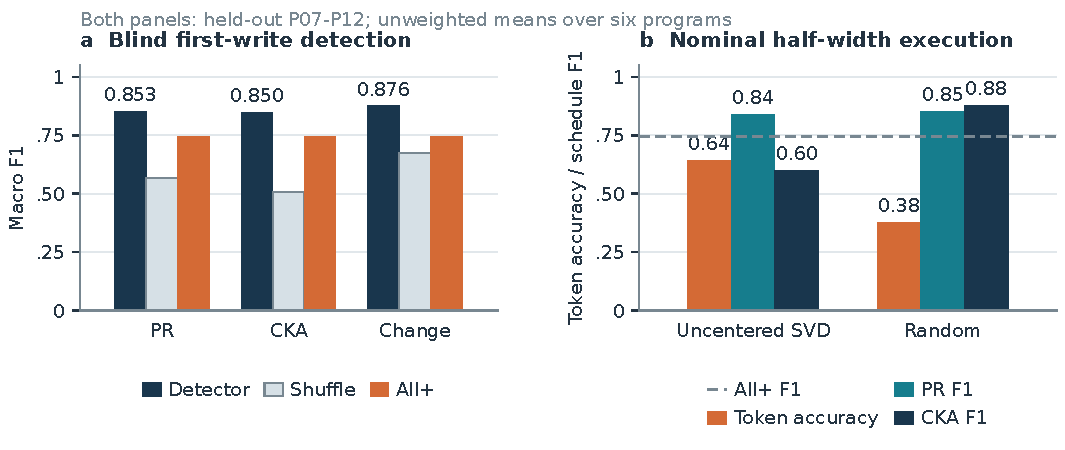
\includegraphics[width=\textwidth]{figures/fig1-recovery-compression.pdf}
\caption{\textbf{Useful timing signals and a failure of interpretation.} Left: blind first-write detection on the six held-out programs, with count-preserving shuffled and always-write baselines. Right: the same held-out group under target half-width compression. A high F1 against the original intended schedule can coexist with poor task accuracy. The schedule is not established causal ground truth for a compressed model whose behavior has changed.}
\label{fig:recovery}
\end{figure*}

\section{Methods}
\lead{Tasks and data.} The twelve tasks include arithmetic, histograms, shifts, order checking, palindrome checking, and sorting. Inputs use the eight integers $-2$ through $5$, length six, and noncausal attention. BOS is excluded from token measurements. The matched fidelity comparison uses 3,383 unique sequences at all six positions, or 20,298 observations per task. Compiled controls use 96 calibration and 96 disjoint test sequences. Learned models use a separate whole-sequence split of 2,029 training, 677 validation, and 677 test sequences.

\lead{Metrics and numerical policy.} For centered representations $X,Y$ with aligned observations and covariance eigenvalues $\lambda_i$,
\begin{align}
\PR(X)&=\frac{(\sum_i\lambda_i)^2}{\sum_i\lambda_i^2},\\
\CKA(X,Y)&=\frac{\|X^\top Y\|_F^2}{\|X^\top X\|_F\,\|Y^\top Y\|_F}.
\end{align}
Linear CKA measures representational similarity~\cite{cka}. Both sides must exceed a total centered sample-variance floor of $10^{-12}$, with ddof~1. Inactive PR is reported as zero by convention; CKA is undefined. Raw spectra, variance, and activity reasons remain saved.

\lead{Representation controls.} Three orthogonal seeds are tested per program. Compression uses an uncentered SVD basis fitted on calibration activations, with rank $\lceil df\rceil$ for original width $d$ and target fraction $f$. Reduced residual streams execute; attention and MLP hidden dimensions remain fixed. Random half-width and full-rank controls are included. A $3\times3$ branch-depth/branch-count family tests structural variation.

\lead{Interventions and blind recovery.} Geometric change selects patch stages using calibration activations. Centered PCA supplies directions; a supervised ridge decoder and compiler candidates subsequently map directions to variables. Test pairs are sampled without requiring different answers. Decoder folds share the calibration PCA fit; final test sequences remain separate. PCA patches are compared with equal-rank random, self, and variable-oracle patches.

Blind detectors receive ordered activation matrices only. Fixed thresholds use residual change energy, PR change, or adjacent CKA change. Predictions are saved and hashed before compiler-schedule scoring. P01 to P06 are the calibration program group and P07 to P12 the held-out group. A 1,000-permutation null preserves each program's predicted event count; an always-write baseline controls for event prevalence. Scores are macro means over programs.

\lead{Learned models.} Twelve tasks and three seeds produce 36 randomly initialized models. All parameters train for 600 Adam steps, with width 32, two layers, two heads, batch size 128, and learning rate 0.003. Learned and compiled stages are paired by relative progress, providing a descriptive geometry comparison rather than variable correspondence.



\begin{figure*}[t]
\centering
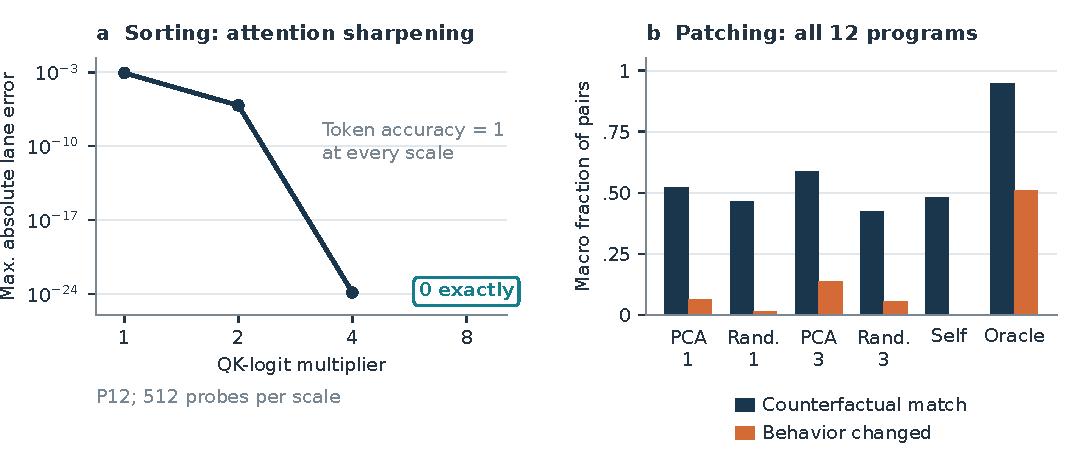
\includegraphics[width=\textwidth]{figures/fig2-attention-patching.pdf}
\caption{\textbf{Numerical diagnosis and geometry-directed interventions.} Left: sharper attention suppresses sorting's lane-amplitude error while decoded accuracy stays 100\%; the recorded zero is shown explicitly. Right: PCA patches show higher symbolic counterfactual agreement than equal-rank random directions and self patches across all twelve programs. Conditions share 192 pairs, and mapping PCA directions to named variables uses labels. These are descriptive comparisons, not independent-sample confidence estimates.}
\label{fig:controls}
\end{figure*}

\section{Results}
\subsection{Numerical artifacts and sorting errors}
The variance floor reduces CKA availability mismatches from 14 to 2 across 54 matched computed-view transitions. Twelve early-stage rows in P07, P08, P10, and P11 have variance about $8.07\times10^{-19}$ despite raw PR near one. The remaining two mismatches involve helper-state versus semantic-state timing. All tested positive floors from $10^{-14}$ to $10^{-8}$ leave two mismatches; the floor is an absolute numerical policy.

With relative and absolute tolerances both $10^{-4}$, sorting's eight output lanes each fail 64 of 512 balanced probes, yielding 87.5\% agreement. The failure sets are disjoint, not a shared failing eighth. Each failed scalar is the target's positive one-hot coordinate. Doubling QK-logit scale reduces maximum lane error from $8.52\times10^{-4}$ to $7.15\times10^{-7}$; at scale eight it is zero. Decoded accuracy remains 100\% throughout (Figure~\ref{fig:controls}). This supports finite-attention approximation, without isolating ties or duplicates as its sole cause.

\subsection{Rotation, compression, and blind recovery}
All 36 executing orthogonal transformations preserve 100\% token and sequence agreement. Maximum posthoc PR and CKA errors are $1.42\times10^{-13}$ and $2.22\times10^{-15}$, while fixed old-lane checks change. Nonorthogonal rescaling changes PR, confirming dependence on feature scale.

Across all twelve programs, SVD compression at target fractions 0.25, 0.5, 0.75, and 1.0 achieves mean token accuracy of 41.30\%, 61.62\%, 72.09\%, and 100\%. Random half-width reaches 37.01\%. Nominal half-width retains a mean 51.77\% of parameters because hidden dimensions remain unchanged. Coordinate overlap is induced; semantic superposition is not independently recovered.

\begin{table}[t]
\centering\small
\caption{Held-out first-write macro F1 on six programs. Shuffled scores preserve predicted event counts.}
\label{tab:recovery}
\begin{tabular}{@{}lrr@{}}
\toprule
Detector & F1 & Shuffled F1\\
\midrule
Residual change & 0.876 & 0.673\\
PR change & 0.853 & 0.567\\
CKA change & 0.850 & 0.506\\
Always write & 0.745 & n/a\\
\bottomrule
\end{tabular}
\end{table}

Blind PR/CKA detectors exceed the always-write baseline on average (Table~\ref{tab:recovery}). The simpler residual-change detector scores higher. P11 CKA scores 0.727, below its 0.737 always-write baseline. More decisively, random half-width compression across the six held-out programs yields CKA intended-schedule F1 0.879 with only 37.62\% task accuracy (Figure~\ref{fig:recovery}). A strong timing score does not guarantee correct execution.



\subsection{Causal, structural, and learned-model controls}
The patch study contains 192 donor-recipient-position pairs and 1,152 correlated condition rows. Rank-three PCA patches match symbolic counterfactuals in $113/192=58.85\%$ of pairs, versus $81/192=42.19\%$ for random rank-three directions and $92/192=47.92\%$ for self patches (Figure~\ref{fig:controls}). They change outputs on 26 pairs. Oracle patches match 182 pairs. Ten undefined P12 substitutions produce 60 failed condition rows across controls; none are discarded.

The nine structural variants have realized depth from 1 to 5, computed-variable count from 1 to 11, and residual width from 24 to 105. Their centered depth/count matrix has rank two, removing the original exact collinearity. Every sampled output agrees with RASP. Serial merges add depth, so branch count is the controlled width factor; these token-local programs do not establish a general complexity law.

For the 36 trained models, per-task mean test token accuracy ranges from 95.41\% to 100\%. Palindrome reaches 95.41\% against a 93.94\% majority baseline, showing why class imbalance matters. Learned final PR is lower than compiled PR for every task; final CKA ranges from 0.152 to 0.802. Matching behavior need not imply matching geometry.

\balance
\section{Discussion and related work}
The controls support partial first-write event recovery. They do not identify variable names, simultaneous write counts, complete algorithms, or the causal computation of changed compressed models. PCA interventions add limited causal evidence, but their semantic mapping is supervised. The absolute variance floor is scale-dependent, trained circuits lack internal ground truth, and neither length/distribution generalization nor erasure/lifetime recovery is established.

The original fidelity benchmark remains useful when labeled accurately. Its full and computed views use aligned observations; the computed view still contains helper lanes. Correlation is retained separately from magnitude: sorting-lane Pearson $r>0.999999999996$ coexists with only 87.5\% tolerance agreement. PR error is a secondary fidelity diagnostic.

Tracr already supports known-structure and superposition experiments~\cite{tracr}. InterpBench~\cite{interpbench} uses Strict Interchange Intervention Training to provide known causal circuits for discovery evaluation. Our ordinarily supervised models do not inherit that internal ground truth. The comparison positions this study; no direct InterpBench benchmark was run.

\section{Conclusion}
Representation geometry reveals some execution timing in controlled transformers. Rotation confirms expected invariance, numerical controls remove misleading scores, and compression supplies a counterexample to interpreting schedule agreement as preserved computation. Stronger algorithm-recovery claims require independent internal ground truth and broader causal validation.

\section*{Data and reproducibility}
Reference runs were recorded 15 October 2026 and pinned to commit \texttt{e06479c}~\cite{artifact}. Saved verification records 28 passing tests, five notebooks with 37 executed cells, and 36 checkpoint replays on 677 test sequences. Manifests preserve dependencies, source hashes, Git state, and failures. No scientific experiment was rerun for this paper.

\begin{thebibliography}{5}
\small\raggedright
\bibitem{tracr} D. Lindner et al. \emph{Tracr: Compiled Transformers as a Laboratory for Interpretability.} NeurIPS, 2023. \href{https://arxiv.org/abs/2301.05062}{arXiv:2301.05062}.
\bibitem{cka} S. Kornblith, M. Norouzi, H. Lee, and G. Hinton. \emph{Similarity of Neural Network Representations Revisited.} ICML, 2019. \href{https://arxiv.org/abs/1905.00414}{arXiv:1905.00414}.
\bibitem{interpbench} R. Gupta, I. Arcuschin, T. Kwa, and A. Garriga-Alonso. \emph{InterpBench: Semi-Synthetic Transformers for Evaluating Mechanistic Interpretability Techniques.} NeurIPS, Datasets and Benchmarks Track, 2024. \href{https://doi.org/10.52202/079017-2950}{doi:10.52202/079017-2950}.
\bibitem{artifact} RaspFormer project. \emph{Canonical implementation and research evidence.} Commit \texttt{e06479c}, 2026. \href{https://github.com/raghulchandramouli/RaspFormer/tree/e06479ce09f10695aa5280162f80d880c060eaf5}{Code, data, predictions, and checkpoints}.
\end{thebibliography}
\end{document}
